\begin{figure}[t]
  \centering
\begin{tikzpicture}[y=.2cm, x=.7cm,font=\sffamily]
 	%axis
	\draw (0,0) -- coordinate (x axis mid) (85,0);
    	\draw (0,0) -- coordinate (y axis mid) (0,5);
    	%ticks
    	\foreach \x in {0,...,85}
     		\draw (\x,10pt) -- (\x,-3pt)
			node[anchor=north] {\x};
    	\foreach \y in {0,1,...,5}
     		\draw (0.01pt,\y) -- (-3pt,\y) 
     			node[anchor=east] {\y}; 
	%labels      
	\node[below=0.8cm] at (x axis mid) {Number of Benchmarks};
  \node[rotate=90, above=0.8cm] at (y axis mid) {Time [seconds]};

	%plots
	\draw plot[mark=*, mark options={fill=white}] 
		file {plotdata/cbmc-time.dat};
	%\draw plot[mark=triangle*, mark options={fill=white} ] 
	%	file {div_ciu.dat};
	%\draw plot[mark=square*, mark options={fill=white}]
	%	file {div_ciu_oscar.dat};
	%\draw plot[mark=square*]
	%	file {div_ciu_oscar_extrapolated.dat};  
    
	%legend
	\begin{scope}[shift={(4,4)}] 
	\draw (0,0) -- 
		plot[mark=*, mark options={fill=white}] (0.25,0) -- (0.5,0) 
		node[right]{soft};
    \Omit{
  \draw[yshift=\baselineskip] (0,0) -- 
		plot[mark=triangle*, mark options={fill=white}] (0.25,0) -- (0.5,0)
		node[right]{ciu};
	\draw[yshift=2\baselineskip] (0,0) -- 
		plot[mark=square*, mark options={fill=white}] (0.25,0) -- (0.5,0)
		node[right]{ciu + oscar};
	\draw[yshift=3\baselineskip] (0,0) -- 
		plot[mark=square*, mark options={fill=black}] (0.25,0) -- (0.5,0)
		node[right]{ciu + oscar extrapolated};
    }
  \end{scope}
\end{tikzpicture}
\caption{\label{fig:results}
  Runtime Comparison between CBMC, Astr{\'e}e and ACDLP}
\end{figure}
